%%%%%%%%%%%%%%%%%%%%%%%%%%%%%%%%%%%%%%%%%%%%%%%%%%%%%%%%%%%%%%%
\chapter{Compiling Instructions}\label{chap:User Manual}
%%%%%%%%%%%%%%%%%%%%%%%%%%%%%%%%%%%%%%%%%%%%%%%%%%%%%%%%%%%%%%%

%\noindent Before you begin to use GEOtop, is advisable you subscribe to the
%users mailing list. By doing it you will receive informations by developers and
%other users, and you will be able to post your question to the community as
%well. Follow the instruction at the following link:\\

%\textcolor{blue}{\underline{{http://www.geotop.org/cgi-bin/moin.cgi/MailinglistUsers}}}\\


\noindent GEOtop runs properly under:
\begin{itemize}
 \item Linux platform;
 \item Mac platform;
 \item Windows platform.
\end{itemize}


%%%%%%%%%%%%%%%%%%%%%%%%%%%%%%%%%%%%%%%%%%%%%%%%%%%%%%%%%%%%%%%
\section{Compile GEOtop through a makefile}
%%%%%%%%%%%%%%%%%%%%%%%%%%%%%%%%%%%%%%%%%%%%%%%%%%%%%%%%%%%%%%%
The GEOtop source code can be downloaded through a terminal (or command prompt if you are using Windows) by typing, 
as shown in \textsl{Figure \ref{cmp}}:\\

\textsl{"svn co https://dev.fsc.bz.it/repos/geotop/trunk/0.9375KMacKenzie"}\\
\begin{figure}[!h]
\begin{center}
  \begin{minipage}[c]{.80\textwidth}
    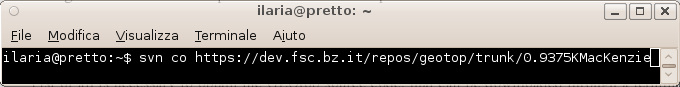
\includegraphics[width=1\textwidth]{./images/pic_compile/compile.png}
    \textsl{\caption{Download GEOtop source code through a terminal} \label{cmp}}
  \end{minipage}
\end{center}
\end{figure}


\noindent The downloaded folder contains the folders:
\begin{itemize}
 \item Debug: which contains the object file created during the compilation and the makefile
 \item geotop: which contains the code
 \item Libraries: which contains the support libraries
\end{itemize}



%\footnotesize{
%\begin{verbatim}
%HM	= .
%LHM		= $(HM)
%BINPATH 	= $(LHM)/
%NAME		= geotop0.9375
%BINS		= $(BINPATH)/$(NAME)

%SCRSPATH1	= $(HM)/KMacKenzie
%LIBPATH1	= $(HM)/LIBRARIES/FLUIDTURTLES
%LIBPATH2	= $(HM)/LIBRARIES/ASCII
%LIBPATH3	= $(HM)/LIBRARIES/GEOMORPHOLOGYLIB
%LIBPATH4	= $(HM)/LIBRARIES/MATH2
%LIBPATH6	= $(HM)/LIBRARIES/KeyPalette
%LIBPATH7	= $(HM)/EXTERN

%OBJ		= 	$(SCRSPATH1)/energy.balance.o $(SCRSPATH1)/frost_table.o\
%		  	$(SCRSPATH1)/geotop.09375.o $(SCRSPATH1)/recovery.o\
%		  	$(SCRSPATH1)/input.09375.o $(SCRSPATH1)/meteo.09375.o\
%		  	$(SCRSPATH1)/output.09375.o $(SCRSPATH1)/pedo.funct.o\
%			$(SCRSPATH1)/radiation.o\
%			$(SCRSPATH1)/snow.09375.o $(SCRSPATH1)/times.o\
%			$(SCRSPATH1)/water.balance_1D.o $(SCRSPATH1)/turbulence.o\
%			$(SCRSPATH1)/water.balance_3D.o $(SCRSPATH1)/vegetation.o\
%			$(LIBPATH1)/alloc.o $(LIBPATH1)/error.o\
%			$(LIBPATH1)/list.o $(LIBPATH1)/t_io.o\
%			$(LIBPATH1)/tensors3D.o  $(LIBPATH1)/utilities.o\
%			$(LIBPATH1)/datamanipulation.o $(LIBPATH1)/random.o\
%			$(LIBPATH1)/linearalgebra.o $(LIBPATH1)/write_dem.o\
%			$(LIBPATH2)/import_ascii.o $(LIBPATH2)/rw_maps.o\
%			$(LIBPATH2)/write_ascii.o $(LIBPATH2)/tabs.o\
%			$(LIBPATH3)/networks.o $(LIBPATH3)/geomorphology.0875.o\
%			$(LIBPATH3)/shadows.o  $(LIBPATH3)/dtm_resolution.o\
%			$(LIBPATH4)/geo_statistic.09375.o $(LIBPATH4)/sparse_matrix.o\
%			$(LIBPATH4)/util_math.o\
%			$(LIBPATH6)/key.palette.o $(LIBPATH6)/get_filenames.o\
%			$(LIBPATH6)/additional_read_functions.o $(LIBPATH6)/read_command_line.o\
%			$(LIBPATH7)/PBSM.o $(LIBPATH7)/micromet.o

%HPATH1 	= $(LIBPATH1)
%HPATH2	= $(LIBPATH2)
%HPATH3  = $(LIBPATH3)
%HPATH4  = $(LIBPATH4)
%HPATH6  = $(LIBPATH6)
%HPATH7  = $(LIBPATH7)
%HPATH0  = $(SCRSPATH1)

%CFLAGS	= -O3 -g 
%INCLUDE = -I$(HPATH1) -I$(HPATH2) -I$(HPATH3) -I$(HPATH4)  -I$(HPATH6) -I$(HPATH7) -I$(HPATH0)

%DEBUG   = -g -Wall
%CC	= gcc $(DEBUG)
%CPP	= g++

%.cc.o: $*.cc $*.h
%	$(CPP) $(CPPFLAGS) -c $< $(INCLUDE) -o $@

%.c.o: $*.c $*.h
%	$(CC) $(CFLAGS) -c $< $(INCLUDE) -o $@

%
%all: geotop

%geotop: $(OBJ)
%	$(CC) -o $(BINS) $(OBJ) -lm -rdynamic -ldl -lstdc++ 
%clean:
%	rm -rf *.o *~ $(OBJ)
%\end{verbatim}
%}

\noindent Open a terminal, go into the folder \textsl{Debug} by typing:

\footnotesize{
\begin{verbatim}
$ cd Debug
\end{verbatim}
}


%By typing \textsl{"ls"} you should have the following files and folders \textsl{Figure \ref{fo}}:
%\begin{figure}[!h]
%\begin{center}
%  \begin{minipage}[c]{.80\textwidth}
%    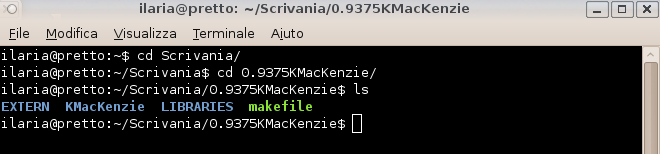
\includegraphics[width=1\textwidth]{./images/pic_compile/folders.png}
%    \textsl{\caption{Necessary files and folders to compile GEOtop through terminal} \label{fo}}
%  \end{minipage}
%\end{center}
%\end{figure}

\noindent To compile GEOtop, type:

\footnotesize{
\begin{verbatim}
$ make all
\end{verbatim}
}

\noindent The executable file {\it GEOtop1.2} is now created in the {\it Debug} folder.

%\textsl{Figure \ref{fo_c}}.\\
%\begin{figure}[!h]
%\begin{center}
%  \begin{minipage}[c]{.80\textwidth}
%    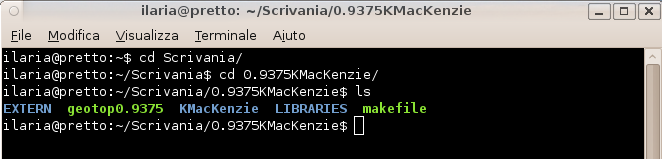
\includegraphics[width=1\textwidth]{./images/pic_compile/folders_compiled.png}
%    \textsl{\caption{Screenshot of the 0.9375KMackenzie folder with the executable} \label{fo_c}}
%  \end{minipage}
%\end{center}
%\end{figure}


%%%%%%%%%%%%%%%%%%%%%%%%%%%%%%%%%%%%%%%%%%%%%%%%%%%%%%%%%%%%%%%%
%\section{Compile and browse GEOtop through Eclipse}
%%%%%%%%%%%%%%%%%%%%%%%%%%%%%%%%%%%%%%%%%%%%%%%%%%%%%%%%%%%%%%%%
%Eclipse is a platform to build integrated development environments (IDEs).
%You first need to download and install it to succesfully compile 
%and browse GEOtop.\\

%\noindent For a complete tutorial download the presentation from:\\

%\textcolor{blue}{\underline{\textsl{http://www.geotop.org/cgi-bin/moin.cgi/Compile\_Instructions}{secondo}}}\\

%\noindent Download and extract the appropriate version for your operative
%system from the following link:\\

%\textcolor{blue}{\underline{\textsl{http://www.eclipse.org/downloads/}{terzo}}}

%
%%=============================================================%
%\subsection{Linux}
%%=============================================================%
%Using Linux Ubunt Karmic Koala 9.10, the Eclipse Galileo release has a bug with the Graphical Interface.
%To fix it follow this instrusctions:\\
%Supposing that the executable file is \textsl{"home\/ilaria\/Scrivania\/eclipse\_folder"},
%create a text file with the following string:\\
%\begin{center}
%  \begin{minipage}[c]{.4\textwidth}
%    \centering
%    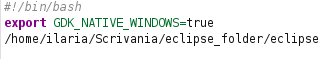
\includegraphics[width=1\textwidth]{./images/pic_compile/0_bug_fix.png}
%  \end{minipage}
%\end{center}
%Save it with a name that you like, but with the extension \textsl{".sh"} in the
%folder where the eclipse executable is, in this example \textsl{"home\/ilaria\/Scrivania\/eclipse\_folder"}.\\
%Right click on the file and allow it to be executable.\\
%Now lunch the .sh file instead of launching the eclipse icon and the bug is
%fixed\\

%%%%%%%%%%%%%%%%%%%%%%%%%%%%%%%%%%%%%%%%%%%%%%%%%%%%%%%%%%%%%%%%
%\subsection{CDT and SVN packages}
%%%%%%%%%%%%%%%%%%%%%%%%%%%%%%%%%%%%%%%%%%%%%%%%%%%%%%%%%%%%%%%%
%You now need to install two packages to succesfully compile GEOtop:
%\begin{itemize}
% \item CDT packages for eclipse Galileo: C/C++ Development Tooling
% \item SVN packages for eclipse Galileo
%\end{itemize}

%\paragraph{CDT packages:}
%\noindent To install the CDT packages go on: \textsl{"Help $\rightarrow$ Install New Software"}
%and in \textsl{"Work with"} add the repository \textsl{"http://download.eclipse.org/releases/galileo"}
%as shown in \textsl{Figure \ref{f:1}}\\
%\begin{figure}[!h]
%\begin{center}
%  \begin{minipage}[c]{.8\textwidth}
%    \centering
%    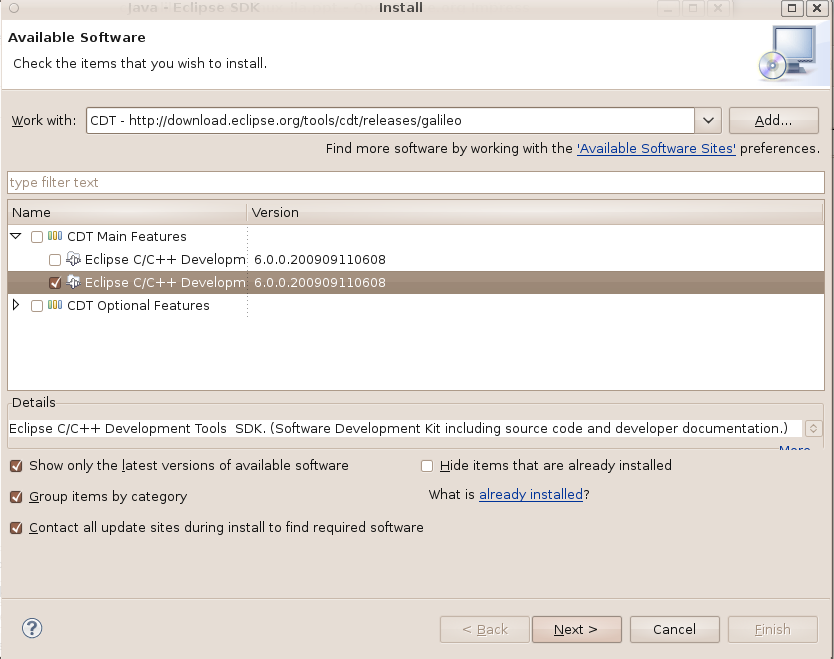
\includegraphics[width=1\textwidth]{./images/pic_compile/2_0_1_update.png}
%    \textsl{\caption{CDT} \label{f:1}}
%  \end{minipage}
%\end{center}
%\end{figure}

%\noindent Click on \textsl{"Next"}. Figure \textsl{\ref{f:2}} shows the packages you 
%are about to install and the license agreement, that you must accept.

%\begin{figure}[!h]
%\begin{center}
%  \begin{minipage}[c]{.45\textwidth}
%    \centering
%    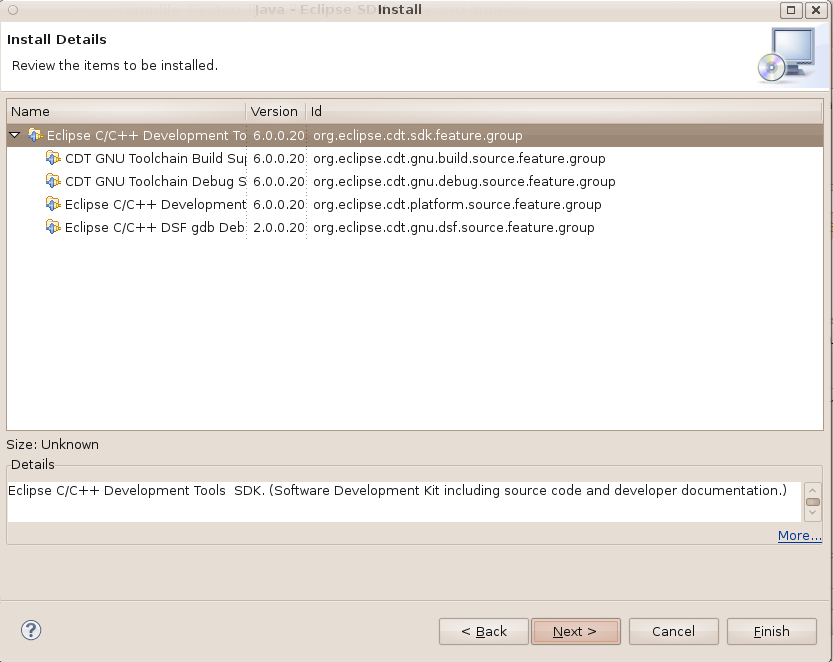
\includegraphics[width=1\textwidth]{./images/pic_compile/2_1_update.png}
%  \end{minipage}
%  \begin{minipage}[c]{.45\textwidth}
%    \centering
%    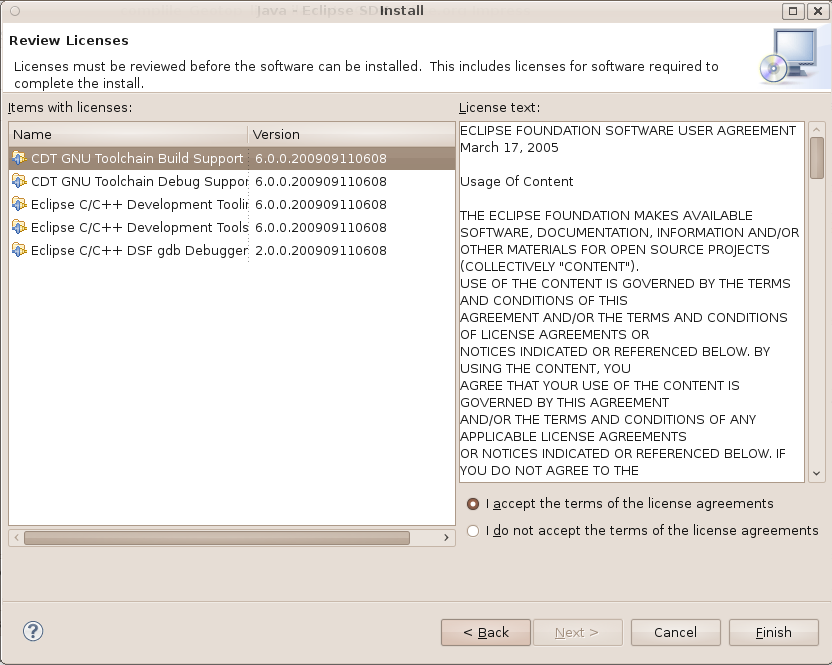
\includegraphics[width=1\textwidth]{./images/pic_compile/2_2_update.png}
%  \end{minipage}
%\end{center}
%    \textsl{\caption{CDT packages and License agreement} \label{f:2}}
%\end{figure}

%%%%%%%%%%%%%%%%%%%%%%%%%%%%%%%%%%%%%%%%%%%%%%%%%%%
%%%%%%%%%%%%%%%%%%%%%%%%%%%%%%%%%%%%%%%%%%%%%%%%%%%
%%%%%%%%%%%%%%%%%%%%%%%%%%%%%%%%%%%%%%%%%%%%%%%%%%%
%\newpage
%\paragraph{SVN packages:}
%\noindent To install the SVN packages go on:
%\begin{itemize}
% \item \textsl{"Help $\rightarrow$ Install New Software"}
%and in \textsl{"Work with"} add the repository \textsl{"http://download.eclipse.org/releases/galileo"}
%check the box \textsl{"Collaboration"} $\rightarrow$ \textsl{"Subversive SVN Team Provider (Incubator)"}
%as shown in \textsl{Figure\ref{f:3}}
% \item \noindent\textsl{"Help $\rightarrow$ Install New Software"}
%and in \textsl{"Work with"} add the repository \textsl{"http://www.polarion.org/projects/subversive/download/eclipse/2.0/update-site"}
%and then choose \textsl{"Subversive SVN Connectors"} $\rightarrow$ \textsl{"SVNKit Implementation (Optional)"}
%as shown in \textsl{Figure \ref{f:3_1}}
%\end{itemize}
% 

%\begin{figure}[!h]
%\begin{center}
%  \begin{minipage}[c]{.45\textwidth}
%    \centering
%    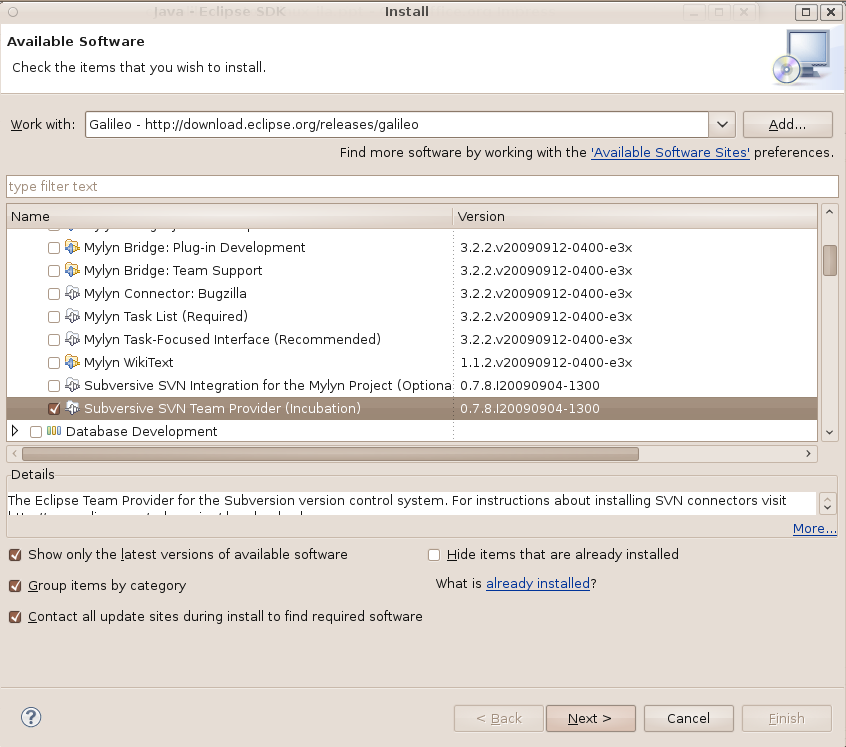
\includegraphics[width=1\textwidth]{./images/pic_compile/3_svn_1.png}
%  \end{minipage}
%%  \begin{minipage}[c]{.45\textwidth}
%%    \centering
%%    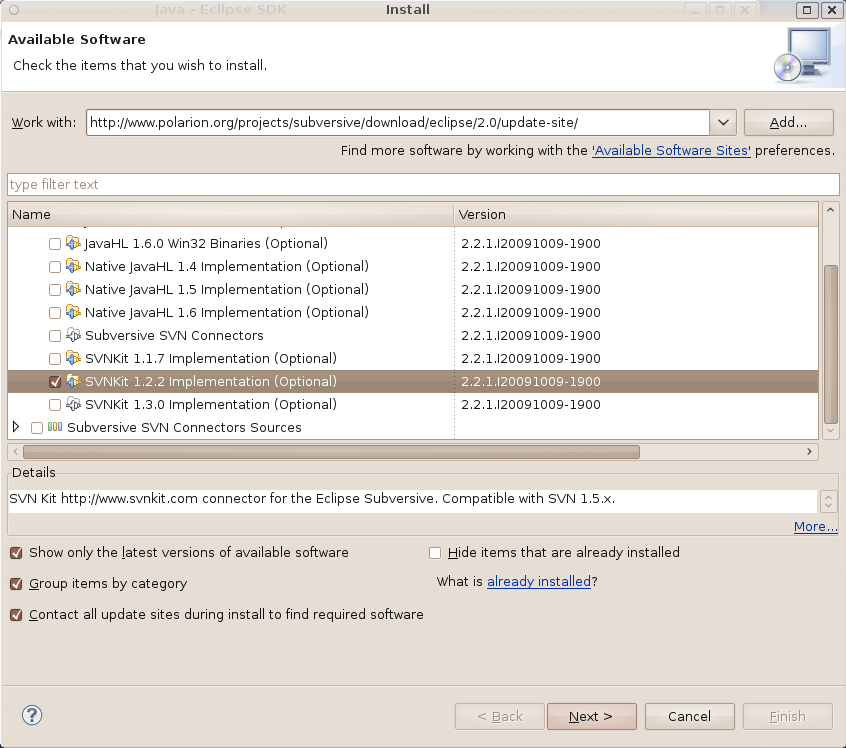
\includegraphics[width=1\textwidth]{./images/pic_compile/3_svn_2.png}
%%  \end{minipage}
%  \end{center}
%    \textsl{\caption{SVN} \label{f:3}}
%\end{figure}

%
%\begin{figure}[!h]
%\begin{center}
%  \begin{minipage}[c]{.45\textwidth}
%    \centering
%    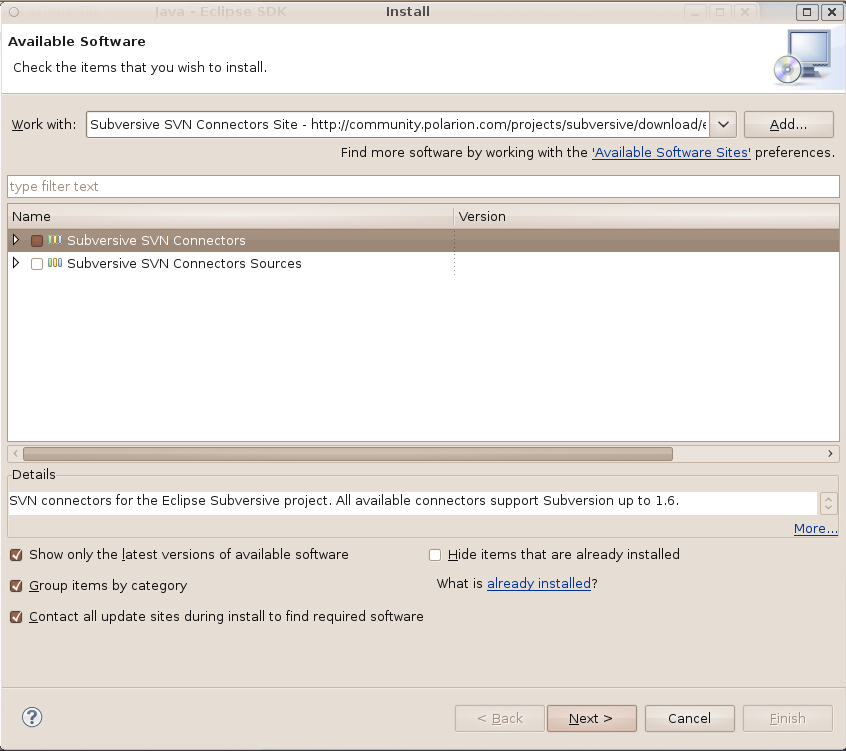
\includegraphics[width=1\textwidth]{./images/pic_compile/3_svn_3.png}
%  \end{minipage}
%  \begin{minipage}[c]{.45\textwidth}
%    \centering
%    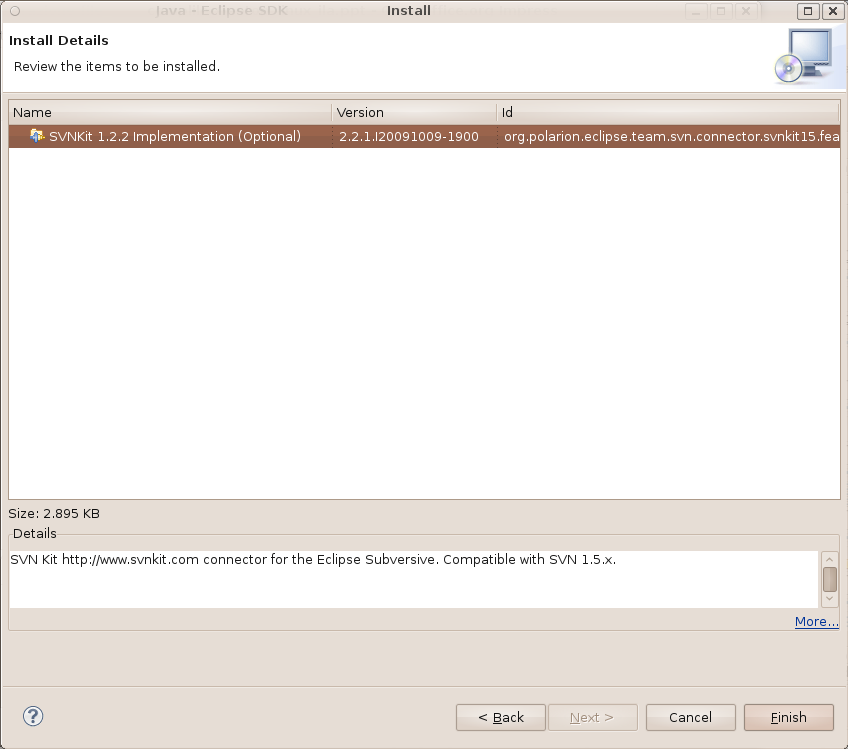
\includegraphics[width=1\textwidth]{./images/pic_compile/3_svn_4.png}
%  \end{minipage}
%  \end{center}
%    \textsl{\caption{SVN} \label{f:3_1}}
%\end{figure}

%

%\clearpage
%%%%%%%%%%%%%%%%%%%%%%%%%%%%%%%%%%%%%%%%%%%%%%%%%%%%%%%%%%%%%%%%
%\subsubsection{Download GEOtop code from SVN}
%%%%%%%%%%%%%%%%%%%%%%%%%%%%%%%%%%%%%%%%%%%%%%%%%%%%%%%%%%%%%%%%
%From \textsl{Window} $\rightarrow$ \textsl{Open prospective} $\rightarrow$ \textsl{Other} $\rightarrow$ \textsl{SVN Repository Exploring} $\rightarrow$ \textsl{OK}\\
%From \textsl{File} $\rightarrow$ \textsl{Import} $\rightarrow$ \textsl{SVN} $\rightarrow$ \textsl{Project from SVN}\\
%Add the Url: \textsl{"https://dev.fsc.bz.it/repos/geotop"} $\rightarrow$ \textsl{"Browse"}\\  
%From \textsl{geotop $\rightarrow$ trunk} $\rightarrow$ select \textsl{"0.9375KMackenzie \#\#"} where the \#\# is the current GEOtop version\\ 
%And then check \textsl{Save in the workspace location path} as shown in \textsl{Figure \ref{f:4}}

%\begin{figure}[!h]
%\begin{center}
%  \begin{minipage}[c]{.4\textwidth}
%    \centering
%    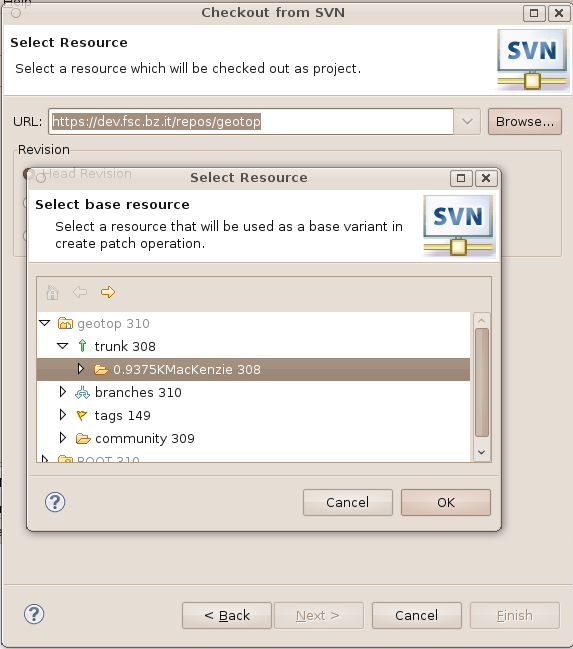
\includegraphics[width=1\textwidth]{./images/pic_compile/3_svn_6.png}
%  \end{minipage}
%  \begin{minipage}[c]{.4\textwidth}
%    \centering
%    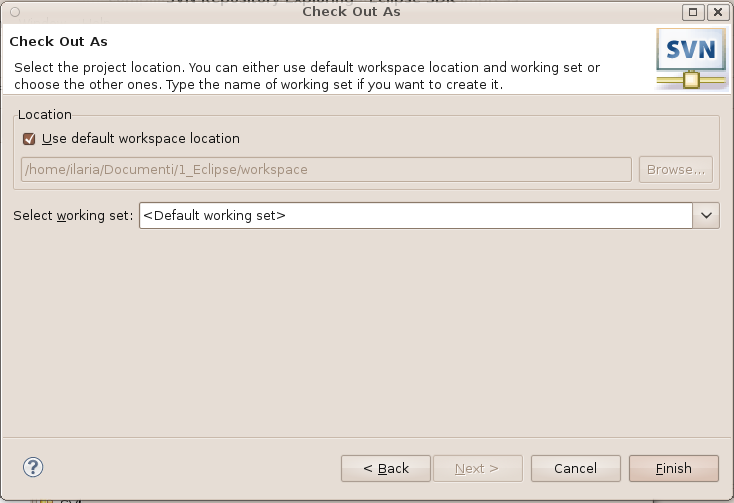
\includegraphics[width=1\textwidth]{./images/pic_compile/3_svn_7.png}
%  \end{minipage}
%\end{center}
%    \textsl{\caption{SVN} \label{f:4}}
%\end{figure}

%\newpage
%\paragraph{Set the C/C++ prospective:}
%%\noindent Set the GNU compiler and math library\\
%From \textsl{Window} $\rightarrow$ \textsl{Open prospective} $\rightarrow$ \textsl{Other} $\rightarrow$ \textsl{C/C++}\\
%The \textsl{'GEOtopKMacKenzie\_SVN'} project will be in the C/C++ prospective \textsl{Figure \ref{f:5}}\\

%\noindent \underline{Linux}\\
%\noindent Right click on \textsl{GEOtopKMackenzie\_SVN folder}
% $\rightarrow$ \textsl{Proprieties}  $\rightarrow$ \textsl{C/C++ Build}  $\rightarrow$ \textsl{Tool Chain Editor}\\
% $\rightarrow$ \textsl{Current Tool chain}: Linux GCC\\
% $\rightarrow$ \textsl{Current builder}: CDT Internal Builder\\

%\noindent Right click on GEOtopKMackenzie\_SVN folder\\
% $\rightarrow$ Proprieties  $\rightarrow$ C/C++ Build  $\rightarrow$ Settings
% $\rightarrow$ GCC C Linker $\rightarrow$ Miscellaneous
% $\rightarrow$ Linker flag: type \textsl{"-lm"} to activate math library \textsl{Figure \ref{f:6}}\\

%
%\begin{figure}[!h]
%\begin{center}
%  \begin{minipage}[c]{.8\textwidth}
%    \centering
%    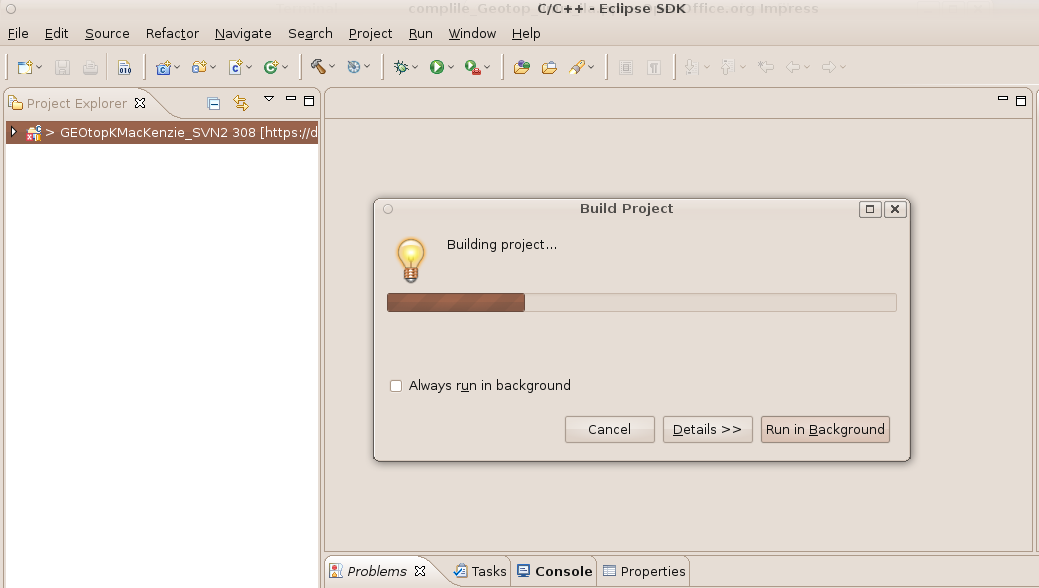
\includegraphics[width=1\textwidth]{./images/pic_compile/7_compile.png}
%  \end{minipage}
%\end{center}
%    \textsl{\caption{SVN} \label{f:5}}
%\end{figure}

%\begin{figure}[!h]
%\begin{center}
%  \begin{minipage}[c]{.4\textwidth}
%    \centering
%    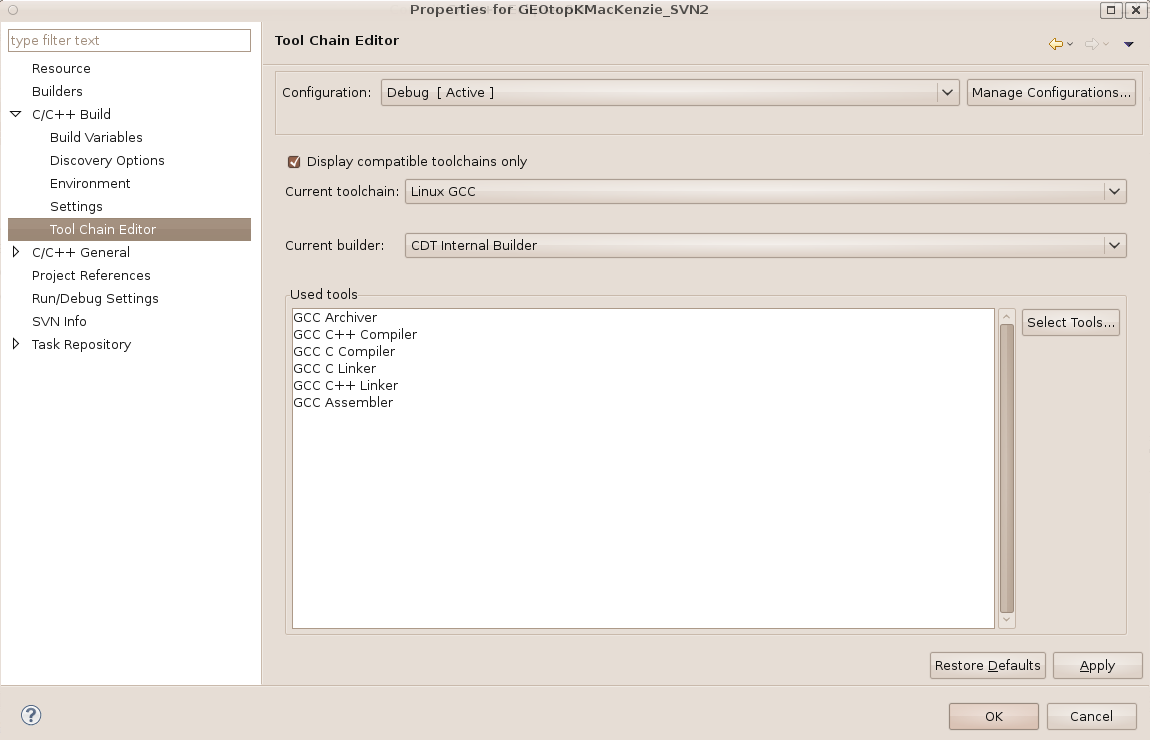
\includegraphics[width=1\textwidth]{./images/pic_compile/Tool_Chain.png}
%  \end{minipage}
%  \begin{minipage}[c]{.4\textwidth}
%    \centering
%    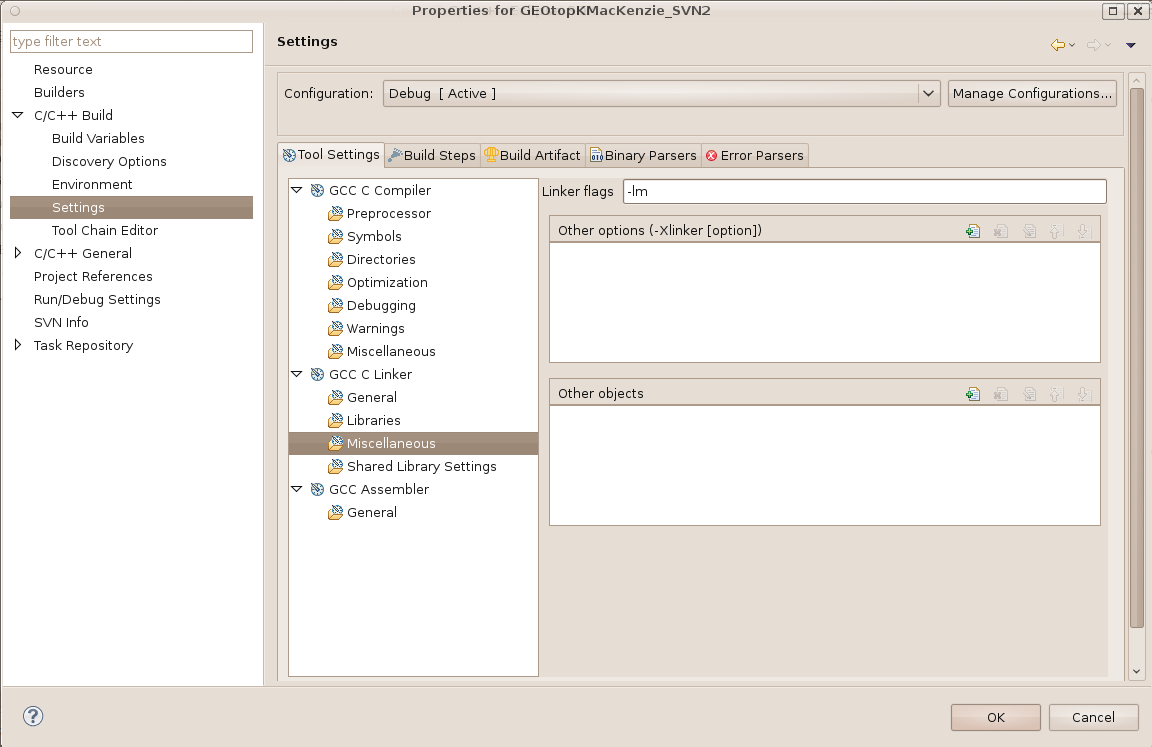
\includegraphics[width=1\textwidth]{./images/pic_compile/Linker_flag.png}
%  \end{minipage}
%\end{center}
%    \textsl{\caption{Tool Chain Editor and Linker Flag} \label{f:6}}
%\end{figure}

%\newpage
%\noindent \underline{MacOSx}\\
%\noindent Right click on \textsl{GEOtopKMackenzie\_SVN folder}
% $\rightarrow$ \textsl{Proprieties}  $\rightarrow$ \textsl{C/C++ Build}  $\rightarrow$ \textsl{Tool Chain Editor}\\
% $\rightarrow$ \textsl{Current Tool chain}: MacOSx GCC\\
% $\rightarrow$ \textsl{Current builder}: GNU Make Builder \textsl{Figure \ref{f:7}}

%\begin{figure}[!h]
%\begin{center}
%  \begin{minipage}[c]{.8\textwidth}
%    \centering
%    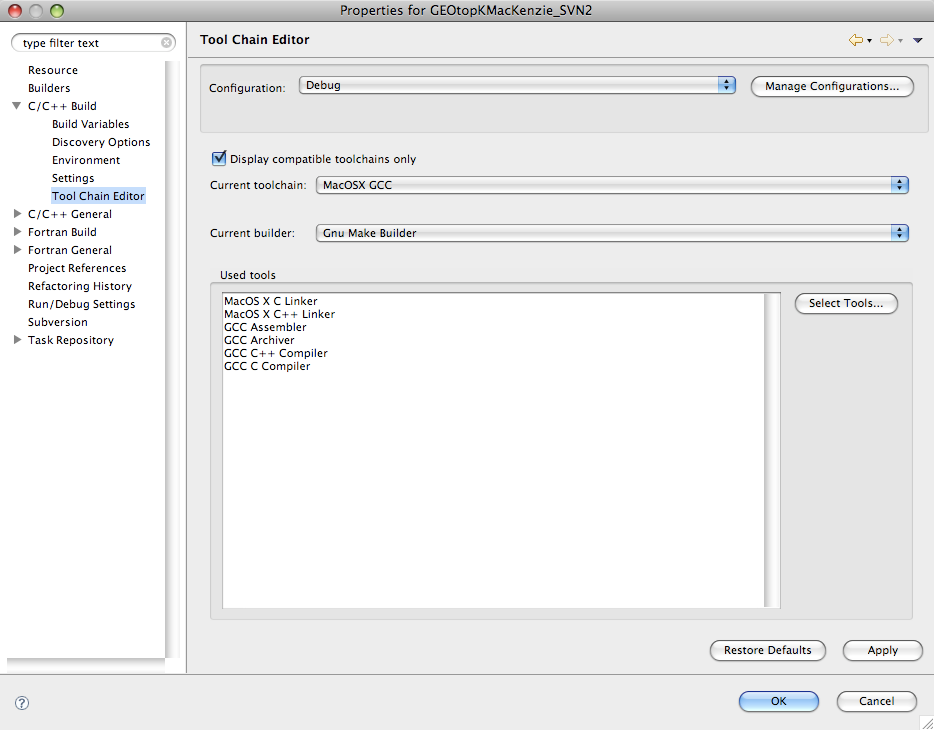
\includegraphics[width=1\textwidth]{./images/pic_compile/screen_Mac.png}
%  \end{minipage}
%\end{center}
%    \textsl{\caption{SVN} \label{f:7}}
%\end{figure}

%\noindent Now is possible to successfully build GEOtop\\
%Click on the hammer symbol: \textsl{Build 'Debug' for project 'GEOtopKMacKenzie\_SVN2'}\\
%GEOtop executable has been built $\rightarrow$ The executable file is under the folder 'Binaries'\\
%\noindent The simulation finished succesfully  \textsl{Figure \ref{f:8}}.

%\begin{figure}[!h]
%\begin{center}
%  \begin{minipage}[c]{.6\textwidth}
%    \centering
%    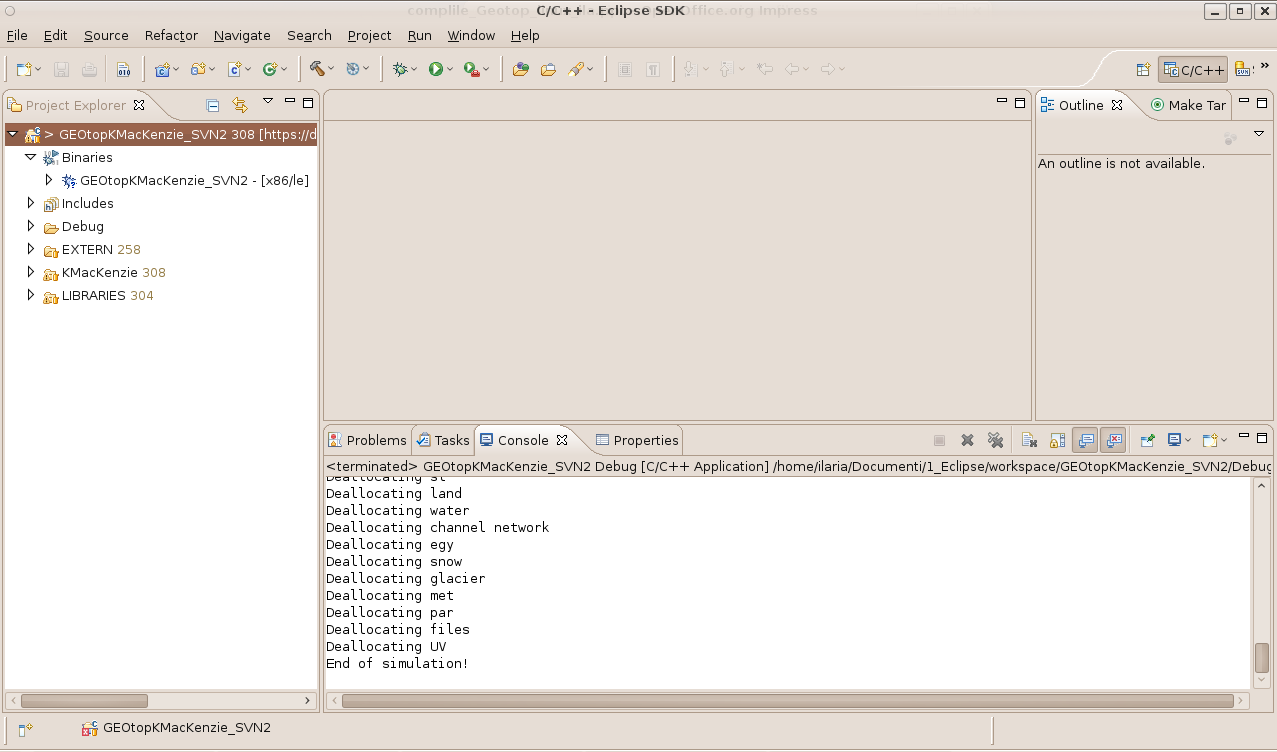
\includegraphics[width=1\textwidth]{./images/pic_compile/12_end.png}
%  \end{minipage}
%\end{center}
%    \textsl{\caption{SVN} \label{f:8}}
%\end{figure}

%

%\newpage
%%%%%%%%%%%%%%%%%%%%%%%%%%%%%%%%%%%%%%%%%%%%%%%%%%%%%%%%%%%%%%%
